%!TEX program = xelatex
%!TEX root = ../thesis.tex
\chapter{GreenEyes Model}\label{chap:greeneyes_model}

In the last chapter, we introduce various works about air pollution and time series forecasting. In our thesis's case, nevertheless, we concern about building an IAQI level evaluation system. When the air pollution level is inferred, the system can drive the peripheral control unit like a purifier to turn on\/off or onto different power levels. Hence, the first problem is to let the system know the current air pollution level and predict the trend. The control feedback can be illustrated as Figure \ref{fig:greeneyes_aiot} shows.

\section{GreenEyes Model}

In our air pollution evaluation system, a regression algorithm is needed to fit the IAQI level curve. Following the preliminaries above, we built our regression model based on WaveNet.

\begin{figure}[!htbp]
    \centering
    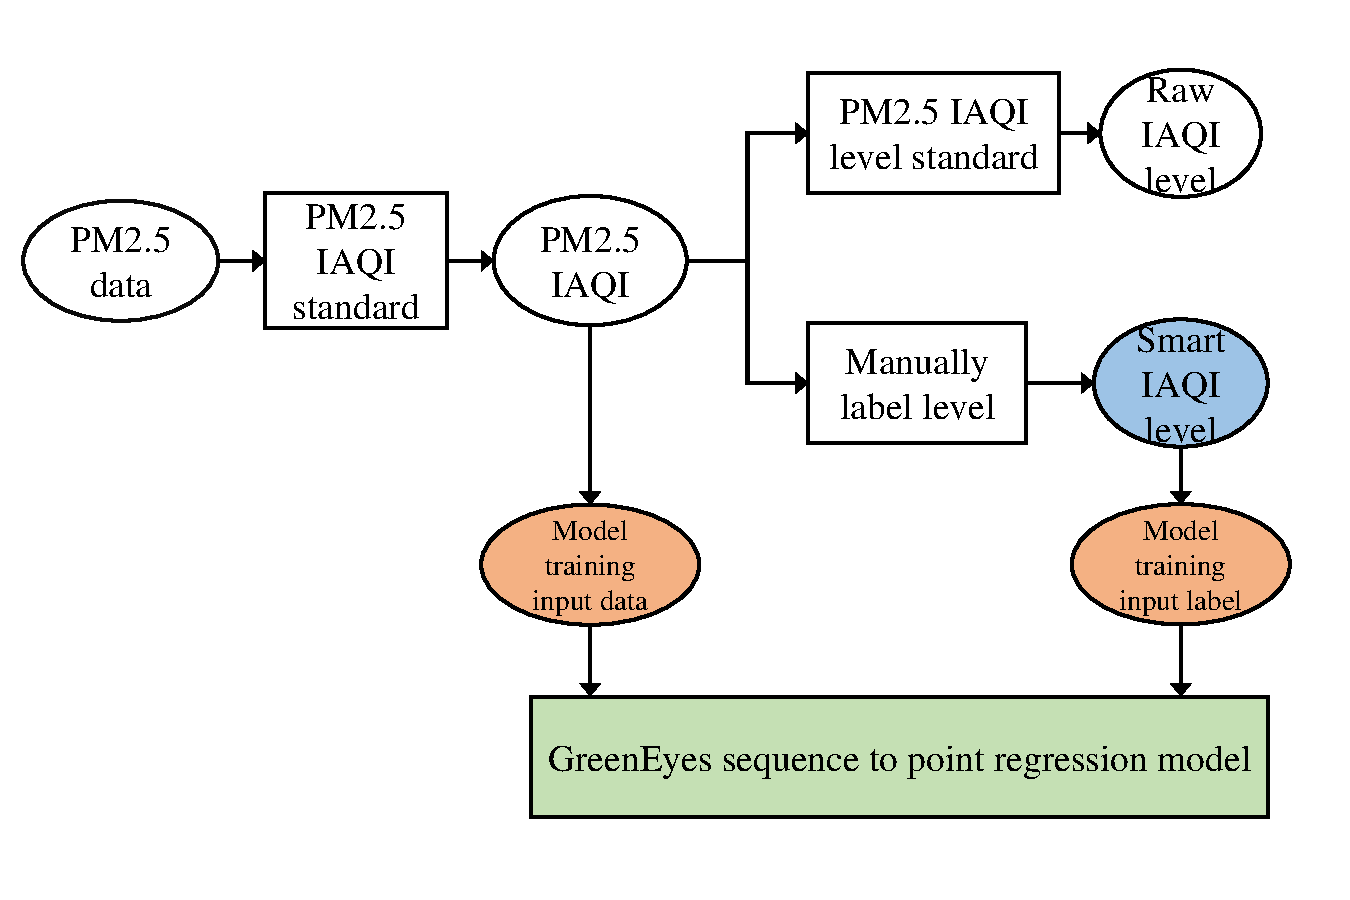
\includegraphics[width=8.3cm]{graphs/greeneyes_pipeline.pdf}
    \caption{Pipeline of the GreenEyes model.}
    \label{fig:greeneyes_pipeline}
\end{figure}

A simple thought of judging some thresholds is only comparing inputs with the border; however, when the inputs fluctuate, especially very acutely, the judge will swing quickly. The collected data may be influenced by noise, shake, and other factors for an economical sensor and a varying environment. Hence, to judge the PM level steadily and dynamically, a smart threshold judging model must be developed. 

\begin{figure}[!htbp]
    \centering
    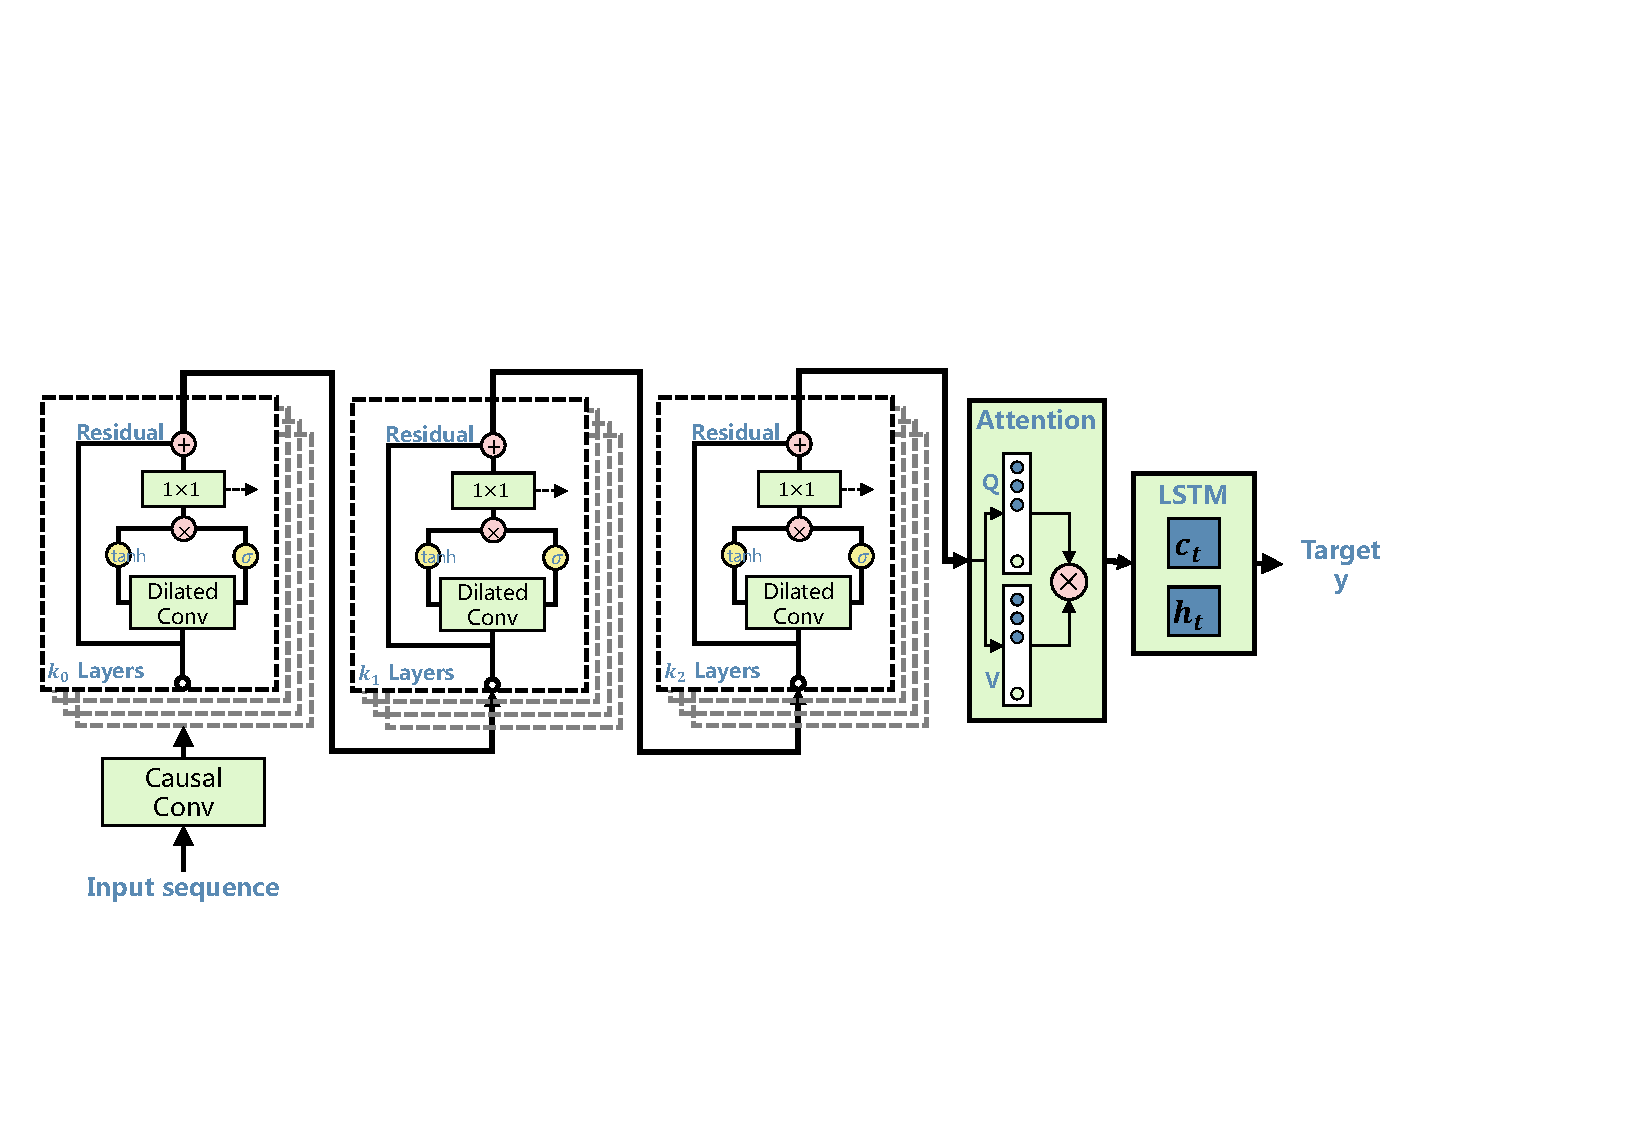
\includegraphics[width=\linewidth]{graphs/WaveNet_LSTM.pdf}
    \caption{GreenEyes sequence to point regression model.}
    \label{fig:greeneyes_model}
\end{figure}

Recently, a series of networks related to audio applications have been developed. DeepMind's WaveNet \cite{oord2016wavenet} is one of the famous. WaveNet used dilated convolution for the sequential inputs and also took advantage of residual connections. We used the original WaveNet's core part as a WaveNet Block. We believe this block\-style configuration is modularized well because we could change these blocks' hyperparameters more easily.

Each WaveNet Block, as the same as WaveNet, contains several dilated convolution layers, called WaveNet Layer. Different dilation rates are also set on them, following DeepMind's original work.

The parameters of our model up to the bottom are list in Table \ref{table:model_parameters}.

\newcommand{\wavenetblockparams}[3]{
  \multirow{3}{*}{
    \(\begin{array}{l}\text{filters=#1}\\\text{kernel\_size=#2}\\\text{wavenet\_layers=#3}\end{array}\)
  }
}
\newcommand{\wavenetblockdetails}[2]{
  \multirow{3}{*}{
    \(\left[\begin{array}{l}\text{Conv1D (1)$\times$#1}\\\text{Conv1D (3)$\times$#1, tanh}\\\text{Conv1D (3)$\times$#1, sigmoid}\end{array}\right]\)$\times$ #2
    }
}
\newcommand{\floor}[1]{\lfloor #1 \rfloor}
\renewcommand\arraystretch{1.1}
\setlength{\tabcolsep}{3pt}
\begin{table*}[t]
\begin{center}
\resizebox{0.8\linewidth}{!}{
\begin{tabular}{|l|l|l|}
    \hline\hline
    Layer & Parameters & Details \\\hline
    \multirow{2}{*}{Conv1D} & \multirow{2}{*}{\(\begin{array}{l}\text{filters=1}\\\text{kernel\_size=1}\end{array}\)} & \\
      &  &  \\ \hline
    \multirow{3}{*}{wavenet\_block} & \wavenetblockparams{16}{3}{8} & \wavenetblockdetails{16}{8} \\
      &  &  \\
      &  &  \\\hline
    AveragePooling1D & pool\_size=10 & \\\hline
    \multirow{3}{*}{wavenet\_block} & \wavenetblockparams{32}{3}{5} & \wavenetblockdetails{32}{5} \\
    &  &  \\
    &  &  \\ \hline
    AveragePooling1D & pool\_size=10 & \\\hline
    \multirow{3}{*}{wavenet\_block} & \wavenetblockparams{64}{3}{3} & \wavenetblockdetails{64}{3} \\
    &  &  \\
    &  &  \\ \hline
    Bidirectional &  &  \\\hline
    Attention & units=7 ($\floor{\frac{7200}{1000}}$) & \\\hline
    Dropout & rate=0.2 & \\\hline
    FC & units=128 & \\\hline
    FC & units=1 & \\
    \hline
    \hline
\end{tabular}
}
\end{center}
\vspace{-.5em}
\caption{The architecture of our GreenEyes model. The number of WaveNet Layer in each WaveNet Block decreases by model depth. Meanwhile, the parameter number of filters increases block by block.}
\label{table:model_parameters}
\vspace{-.5em}
\end{table*}
